\chapter{浏览器——网上冲浪必备}
\label{cha:browsers-and-how-to-choose}

\begin{intro}
  浏览器是我们浏览网页的必备工具,它们将互联网上的形形色色的网页呈现在我们面前。不过,各种浏览器之间的门派以及它们之间交错复杂的历史渊源,却并不为多数人所知。阅读完本章,你也许可以找到下面这些问题的答案。
  
  \begin{itemize}
    \item IE 浏览器是何方神圣?
    \item Chrome 浏览器又是何方神圣?
    \item 火狐浏览器又是何方神圣?
    \item 「360 安全浏览器」「QQ 浏览器」都是怎么来的?
    \item 我应该选择什么浏览器?
  \end{itemize}
\end{intro}

想要「网上冲浪」?浏览器必不可少。当你尝试访问一个网站时,浏览器会向对应网站的服务器发送请求。一旦服务器传回了网页内容,浏览器就会将这些内容按网站的要求「排版」,使其能完整、正确地展现在你的屏幕上。同时,浏览器还负责与你交互:假如你点了一下这个网站上的某个按钮,浏览器就要去「理解」你的点击动作,并执行相应的功能。

\begin{figure}[htb!]
  \centering
  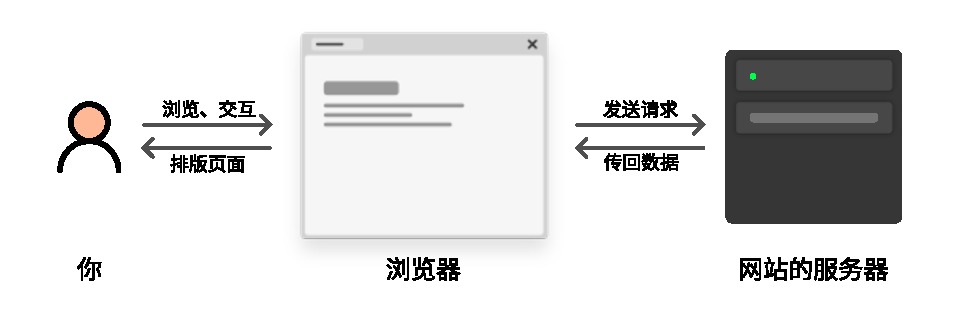
\includegraphics[width=.95\textwidth]{assets/software/How_browser_works.pdf}
  \caption{浏览器干的事}
  \label{fig:How_browser_works}
\end{figure}

正如有人做题做得快,有人做得慢,排版同一个网页,有的浏览器排得又快又好,有的则要花费更长的时间。浏览器之间的最直观区别,就体现在同一网络下打开网页的不同速度上。当然,不同的浏览器也有自己的特色,有的可以帮忙屏蔽一些广告,有的可以帮你记忆各种密码,有的能与自家的「电脑管家」联动来保障安全,有的则只被用来下载其他浏览器。「IE 浏览器」「火狐浏览器」「谷歌浏览器」「360 极速浏览器」「QQ 浏览器」……这些名字或许你早已有所耳闻,但它们究竟孰优孰劣,可能还需要深入了解才能知晓。

\section{浏览器界的「血雨腥风」}

在讨论浏览器之前,我们可以先侃一侃「浏览器战争史」。

\subsection[第一次浏览器大战——网景和微软两大巨人的单打独斗]{第一次浏览器大战{\normalsize ——网景和微软两大巨人的单打独斗}}

让我们将时间的指针拨到 30 年前。二十世纪九十年代,互联网刚刚进入民用领域,市面上开始出现各种各样的早期网络浏览器,它们的出现为一场「没有硝烟的战争」拉开了序幕。

\begin{wrapfigure}{r}{5cm}
  \centering
  
\includegraphics[width=4cm]{assets/software/Netscape_logo.png}
  \caption{网景公司的 logo}
  \label{fig:Netscape_logo}
\end{wrapfigure}

这些早期浏览器的作者中,有一个叫马克·安德森(Marc Andreessen)的人比较有商业头脑——他嗅到了互联网时代的机遇。1994 年,他和自己的伙伴成立了「网景通讯」(Netscape Communications)公司,并推出了一款商业化的浏览器软件——「\regcolor{网景浏览器}」(Netscape)。网景浏览器以「共享软件」的方式运作——即软件本身需要交钱购买,但是可以先免费试用。由于网景浏览器相比竞品(虽说那时本来也没什么竞品)更加实用、稳定,网景很快统领了浏览器的市场,并成为了互联网领域的「绝对标准」。右图是网景浏览器的 logo。

微软见网景在互联网领域如鱼得水赚了大钱,心里很不是滋味,于是也想在浏览器领域分一杯羹。1995 年,微软发布了「Internet Explorer」,它简写来就是「IE」。IE 在一开始并没有取得什么竞争上的优势。当时的它,不如网景浏览器稳定,反而有着更多的安全漏洞,更容易导致死机。但到了 1997 年,微软发布 IE 4.0,这个版本的 IE 做了几件大事:一是\regcolor{它变成了 Windows 系统中的一部分}\CJKsout*{(捆绑安装)},二是它终于做得比网景更好了。自此之后,IE 迅雷不及掩耳地抢占了大量市场份额。到了 1998 年,网景被一家美国公司「美国在线」(简称 AOL)收购,原来的浏览器开发团队也解散了。下面是 IE 4.0 的软件界面:

\begin{figure}[htb!]
  \centering
  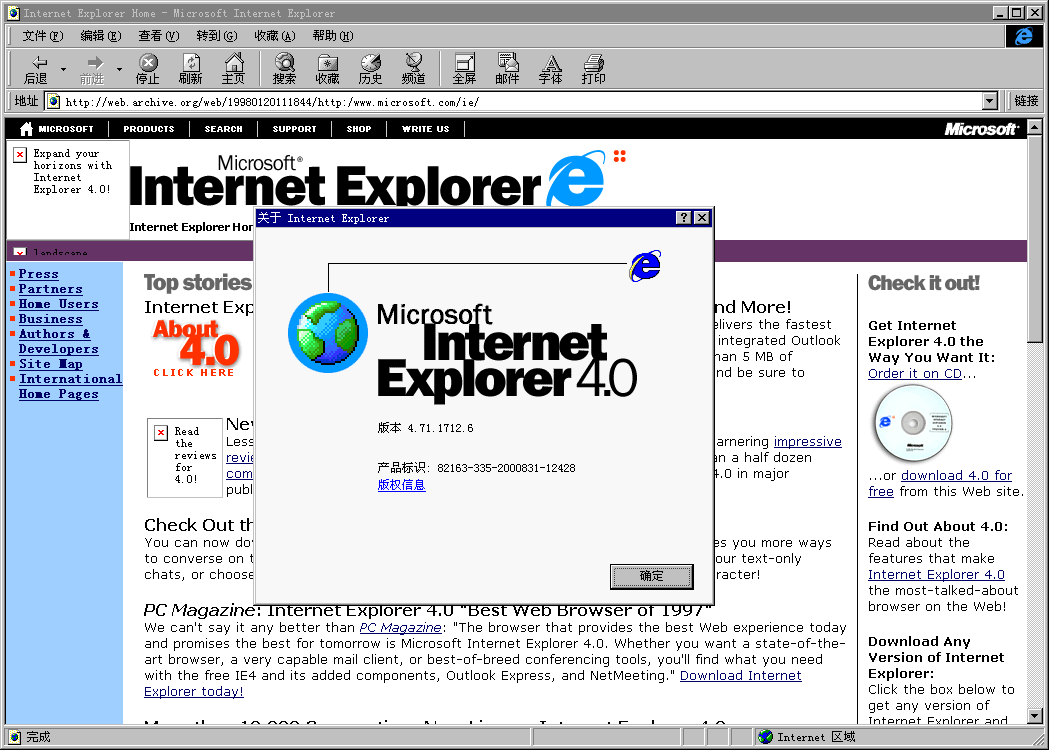
\includegraphics[width=.75\textwidth]{assets/software/IE4.png}
  \caption{IE 4.0 的界面}
  \label{fig:IE4}
\end{figure}

至此,微软在这一场与网景的较量之中胜出,IE 浏览器成为了浏览器界的老大,第一次浏览器大战结束。

\subsection[第二次浏览器大战——开放、自由的竞争与新时代的机遇]{第二次浏览器大战{\normalsize ——开放、自由的竞争与新时代的机遇}}

网景虽然在第一次浏览器大战中惨败,但它并没有立刻退出这个市场,而是希望联合更多的力量来抗衡自己的对手。1998 年,也就是网景被收购的那年,它\regcolor{公开了自己的网景浏览器的源代码,成立了以 Mozilla 为名的开发社团},希望借助更多人的力量将这一股薪火传下去。

时间来到 2003 年,苟延残喘的网景公司最终解散。解散当天,AOL 也分离了与 Mozilla 的关系,Mozilla 成了一个独立的基金会。所谓「基金会」,就是说自身不以营利为目的,而依赖社区——或者说大众——的力量进行开发,依赖用户的捐赠来维持运行。不久后,\regcolor{Mozilla 将自己开发的,「传承」自网景的浏览器赋予「Firefox」的名字,即「火狐」}。下图便是当时 Firefox 的界面。由开放社区贡献的 Firefox 得到了人们的认可,数年间就占领了超过 20\% 的浏览器市场。

\begin{figure}[htb!]
  \centering
  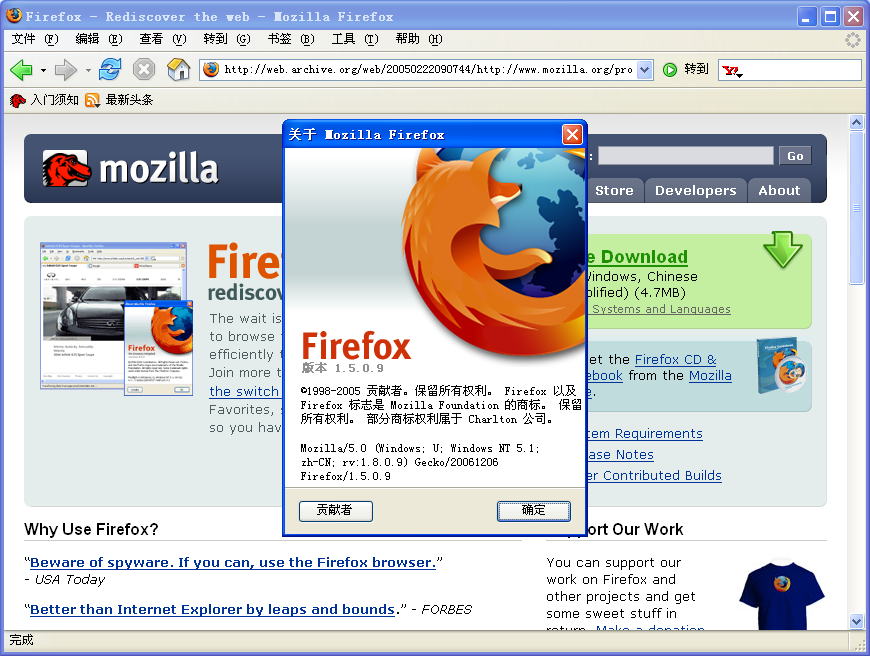
\includegraphics[width=.6\textwidth]{assets/software/Firefox_1.5.png}
  \caption{Firefox 1.5 的界面}
  \label{fig:Firefox_1.5}
\end{figure}

微软见 Firefox 迅速占领市场,来者不善,于是着手为 IE 添加新的功能,以让它能与 Firefox 抗衡。2006 年,微软发布了 IE 7,在界面和功能上都有了许多改变,但却在性能上惨不忍睹,在新标准支持方面也实在难以恭维。又由于为 IE 7 护航的 Windows Vista 在市场上完全失败,IE 7 几乎没有取得什么成功。后来的 IE 8 尽管做了很大改进,但在新标准支持方面仍然表现差劲,与竞争对手间存在很大的差距。IE 的市场份额因而不断走向下坡,而 Firefox 的占有率则在 2008 年前后冲上了 30\% 的高峰。

\begin{figure}[htb!]
  \centering
  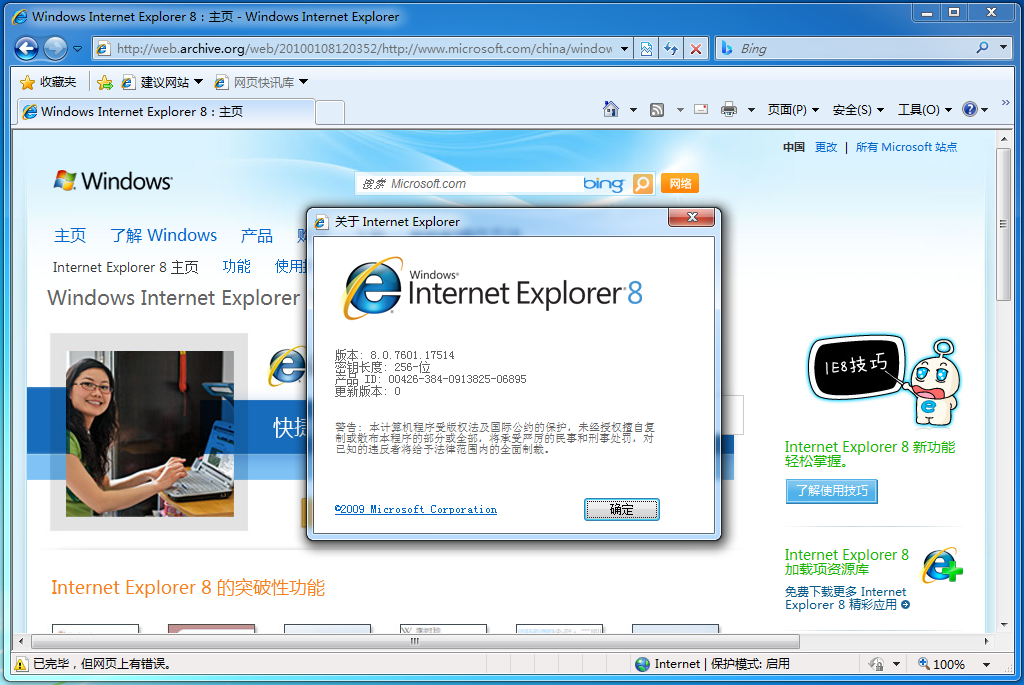
\includegraphics[width=.6\textwidth]{assets/software/IE8.png}
  \caption{IE 8 的界面}
  \label{fig:IE8}
\end{figure}

与此同时,越来越多的企业和组织意识到了浏览器市场的重要性。除了 Mozilla 的 Firefox 和微软的 IE 外,其他许多竞争者也参与到了这场新的浏览器大战中。2008 年,\regcolor{美国科技巨头谷歌推出了一款全新浏览器——Chrome 浏览器,也就是我们俗称的「谷歌浏览器」}。下面便是早期 Chrome 浏览器的界面。

\begin{figure}[htb!]
  \centering
  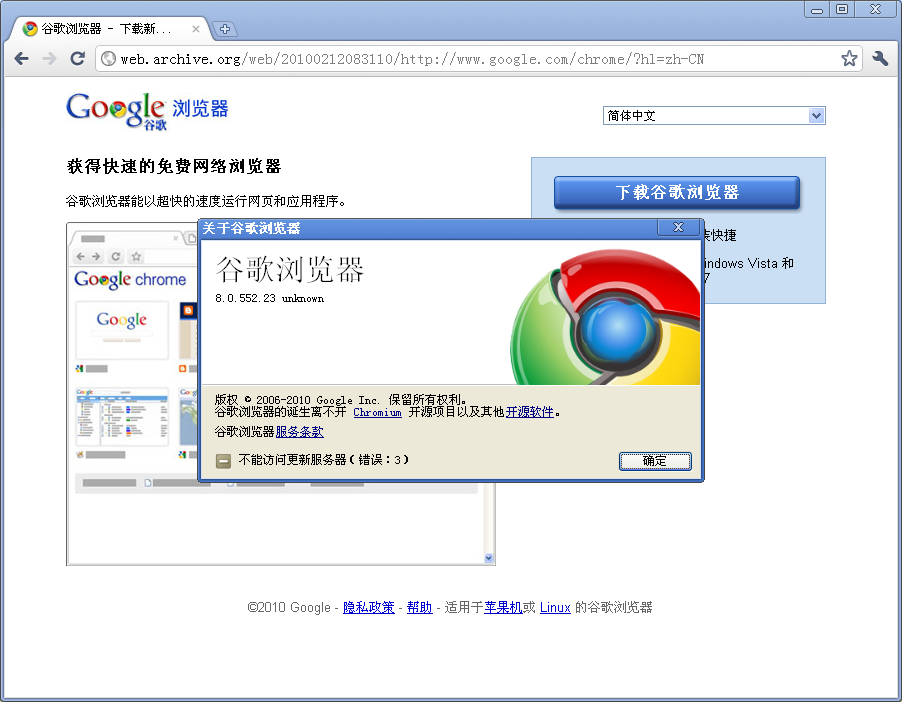
\includegraphics[width=.7\textwidth]{assets/software/Chrome_8.png}
  \caption{Chrome 8 的界面}
  \label{fig:Chrome_8}
\end{figure}

Chrome 浏览器诞生不久就开始迅猛发展并占领市场。这有着多方面的原因:第一,谷歌自身的体量强大,因而能够借助自己的网络生态——例如谷歌搜索、谷歌邮箱(Gmail)等访问量巨大的网站——来助推 Chrome 浏览器。第二,谷歌的确投入了人力物力进行 Chrome 浏览器的开发,一直以来,Chrome 浏览器在性能上与竞争对手相比都有着不小的优势。

\begin{note}
  另一个重要原因是,Chrome 浏览器诞生的年代(2010 年前)正好是赶上了互联网从原来的单一化向多元化发展的时代大潮。而 Chrome 对那时产生的一系列新标准和规范有较好的支持,可以说是一直赶在时代潮头;相比之下,由于微软的 IE 浏览器是与 Windows 系统捆绑更新的,而 Windows 系统数年才发布一个新版本,再加上 IE 无论是性能还是功能都不断地落后于其他浏览器,IE 的市场占有率自那时开始就持续走低。
\end{note}

前面我们提到过,Firefox 是开源的软件,它的源代码自诞生以来一直都是公开的——这意味着,任何人都可以在遵守一定约定的前提下,自由地修改和发布它。这样,Firefox 就能「集思广益」,以社区之力推进开发。谷歌看到了这种模式的优势,但又不想让自己的得意之作完全被众人窥探,于是谷歌想了个办法,它\regcolor{将 Chrome 浏览器的核心部分拿出来,以「Chromium」这个名字开源}\footnote{「Chrome」是「铬金属」,「Chromium」是「铬元素」,外在与内核,正是照应了它们的名字。}。有了 Chromium,社区大众可以拿它去进行二次开发和改进,谷歌则将这之中的开发进展不断地吸收回 Chrome。这样就形成了「由开放的 Chromium 反哺封闭的 Chrome」的过程。如果你正在使用 Chrome 浏览器,不妨点击右上角的【\makebox[.8em]{⁝}】,选择【设置】→【关于 Chrome】,你就能看到这样一句话:「Chrome 的诞生离不开 Chromium 开源项目以及其他开源软件」。

\begin{figure}[htb!]
  \centering
  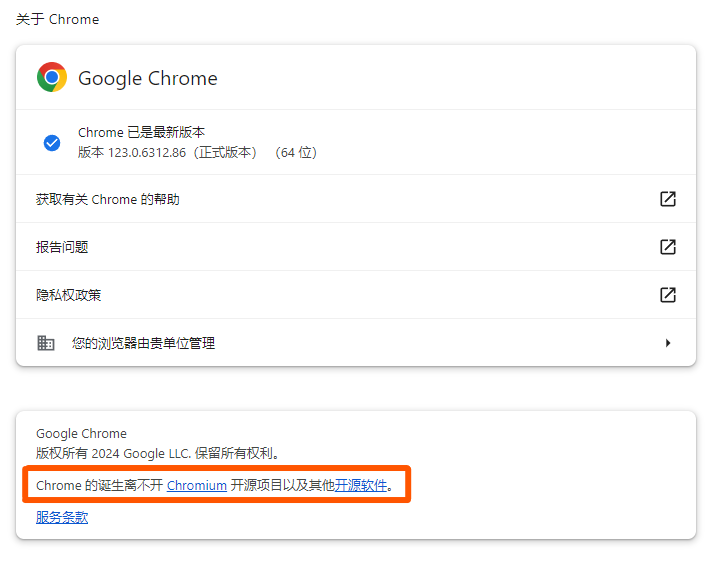
\includegraphics[width=.8\textwidth]{assets/software/About_chrome.png}
  \caption{关于 Chrome 页面}
  \label{fig:About_chrome}
\end{figure}

众所周知,Chrome 浏览器好用,而谷歌又把它核心部分给公开了,这让许多其他厂商有了新的想法:从零开始重新设计一个浏览器实在太难,但浏览器着实赚钱(主要是广告效应,以及可以借浏览器来推广自家的其他功能),不如就\regcolor{把这 Chromium 借来,套上一个外壳,加上一些小功能,做成自己的浏览器}好了。由于国内特殊的网络环境,谷歌的一些服务在中国内地无法使用,这更给予了国内一些互联网大厂打造自己浏览器的动力。「360 极速浏览器」「QQ 浏览器」等等这些国产浏览器,都是在 Chromium 的基础上套壳而来的产物——它们都使用着和 Chrome 一样的核心,只是披上了不同的外衣,附加了各自的独有功能。在这些浏览器的有关页面上,我们也都能找到它们与 Chromium 的关系。例如,下图是 360 极速浏览器的介绍页,这里的「Chrome 内核」指的就是 Chromium。

\begin{figure}[htb!]
  \centering
  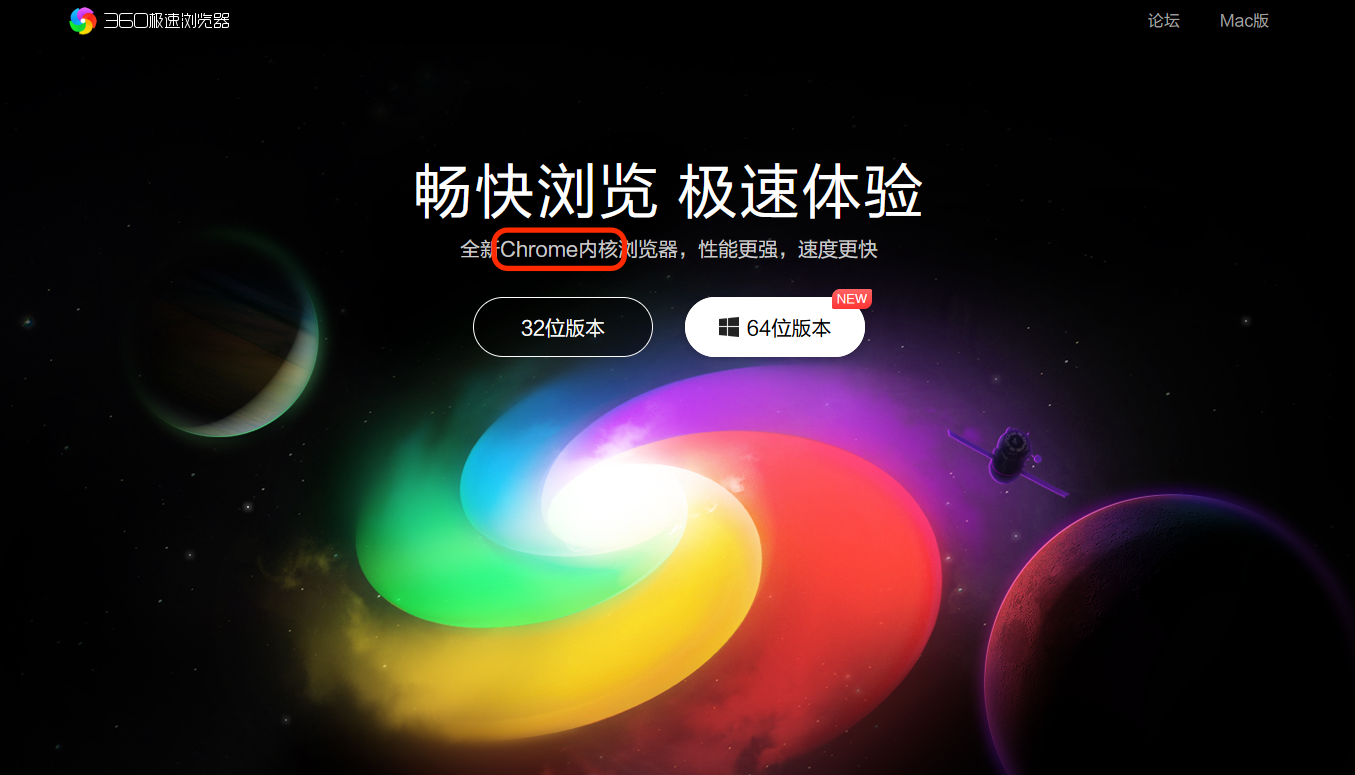
\includegraphics[width=.9\textwidth]{assets/software/360_ee.png}
  \caption{360 极速浏览器}
  \label{fig:360_ee}
\end{figure}

再比如说,QQ 浏览器的「关于」页面中就写明了此版本浏览器所依赖的 Chrome 内核版本,呃,以及 IE 内核版本\CJKsout*{(不过现在 Chromium 都版本 120+ 了你怎么还在用 94 啊?)}。

\begin{figure}[htb!]
  \centering
  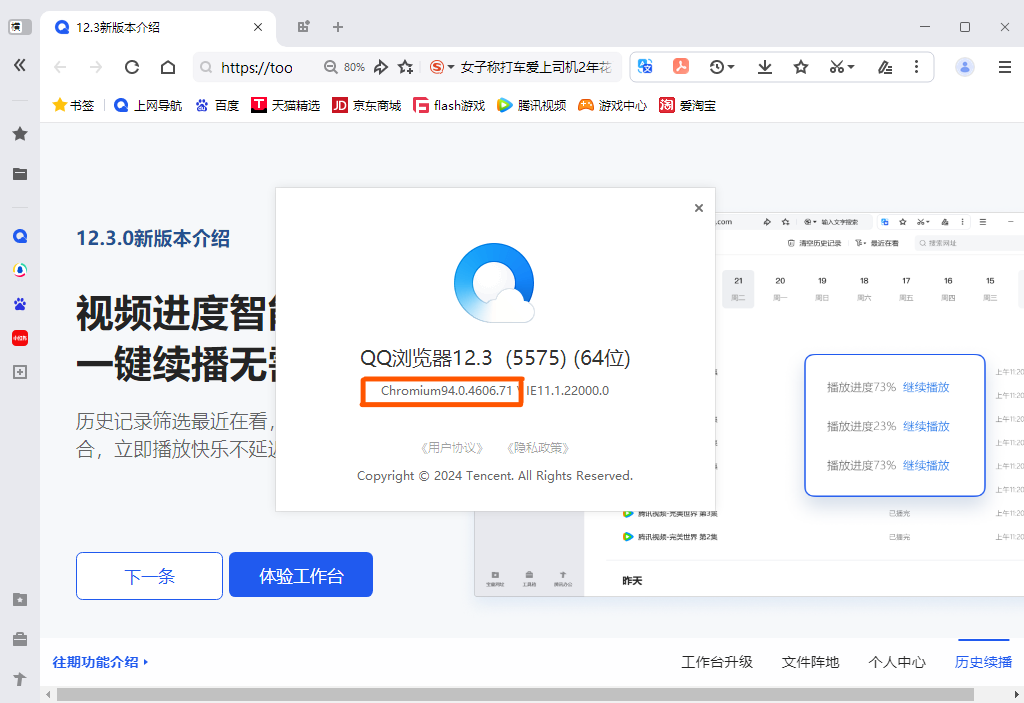
\includegraphics[width=.6\textwidth]{assets/software/QQ_Browser.png}
  \caption{QQ 浏览器的「关于」页}
  \label{fig:QQ_Browser}
\end{figure}

就连微软——又是你微软——也在最后走上了套壳 Chromium 的道路。先回头看看 IE 浏览器,它自 2013 年的 IE 11 以来就没有再更新过大版本。倒是在 2015 年前后,微软发布了一款新的浏览器「Edge」,彼时的 Edge 还是在 IE 的基础上开发的,可以算是 IE 的正统后继者——连 IE 的缺点也一并后继了。于是之后几年,Edge 一直不温不火,尽管它和 Windows 10 捆绑,但市场占有率一直比较低迷。\CJKsout*{毕竟 IE 的底子实在太差,那几年的 Edge 只能说稍微比过去的 IE 好那么一丁点。}

\begin{wrapfigure}{r}{6cm}
  \centering
  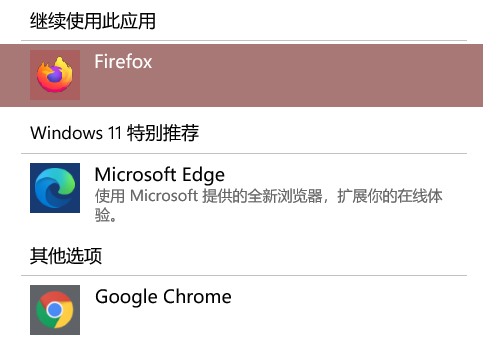
\includegraphics[width=5.3cm]{assets/software/Windows_11_suggesting_Edge.png}
  \caption{「来试试Edge吧!」}
  \label{fig:Windows_11_suggesting_Edge}
\end{wrapfigure}

时间一转眼到了 2018 年。那年末,微软搞了一个大新闻,要将 Edge 迁移到 Chromium 内核——换句话就是,把 Edge 原来的技术扔掉不要,新的 Edge 将是一款 Chromium 套壳的浏览器。\regcolor{新 Edge 最终在 2020 年正式问世,全称「Microsoft Edge」}\hspace{-.5em}\CJKsout*{(微软边缘)}。这或许是微软的一次翻身——近两年,Edge 浏览器的市场份额开始稳步上升,一方面得益于 Chromium 内核的强大,另一方面则是微软借 Windows 来强行推荐 Edge。如果你使用的是 Windows 10 或 11,你一定在系统的许多地方都能看见微软强行推荐 Edge 的身影:

而 IE 真的成为弃子了:目前,许多网站(包括《你缺计课》网页版)已经无法使用 IE 浏览器正常打开;Windows 11 和 10 均已隐藏了 IE 浏览器的入口。诞生于第一次浏览器大战的 IE 在那时碾压对手网景,却最终在第二次浏览器大战中成为历史。在今天,除了因国内有一些网站由于这样那样的历史原因必须要使用 IE 浏览器才能正常工作外,我们已经没有任何理由去使用 IE 浏览器。

\begin{note}
  尽管 IE 已经被这个时代抛弃,但每个时代都有自己的「IE」——今天苹果的 Safari 浏览器,就和过去的 IE 有着一样的毛病:与系统捆绑更新;对漏洞的修复并不及时,对新标准的支持并不完整;功能欠缺,扩展性弱……更令人不齿的是,苹果在移动设备(即 iOS 和 iPadOS)上强制所有第三方浏览器使用 Safari 内核,完全剥夺了用户的选择权。可惜,由于苹果财大气粗,即使其与时代之势背道而行,孤行己见,目中无人,Safari 在短期内也不会有像 IE 那样的命运。
\end{note}

\autoref{fig:Browser_market_share} 展示了知名网络流量分析公司 Statcounter 发布的 2009 至 2024 年间全球电脑浏览器市场份额变化情况。从图中可以看到,Chrome 浏览器自发布以来市场份额迅速攀升,自 2019 年起便稳定维持在 70\% 左右;而基于 Chromium 内核的新 Edge 浏览器同样自推出后迅速占领市场,并在发布仅两年后便获得了 10\% 的份额。两者合计占据了超过 80\% 的市场份额,再加上各类基于 Chromium 内核的套壳浏览器,称 Chrome 浏览器几乎垄断了电脑浏览器市场,毫不为过。

\begin{figure}[htb!]
  \centering
  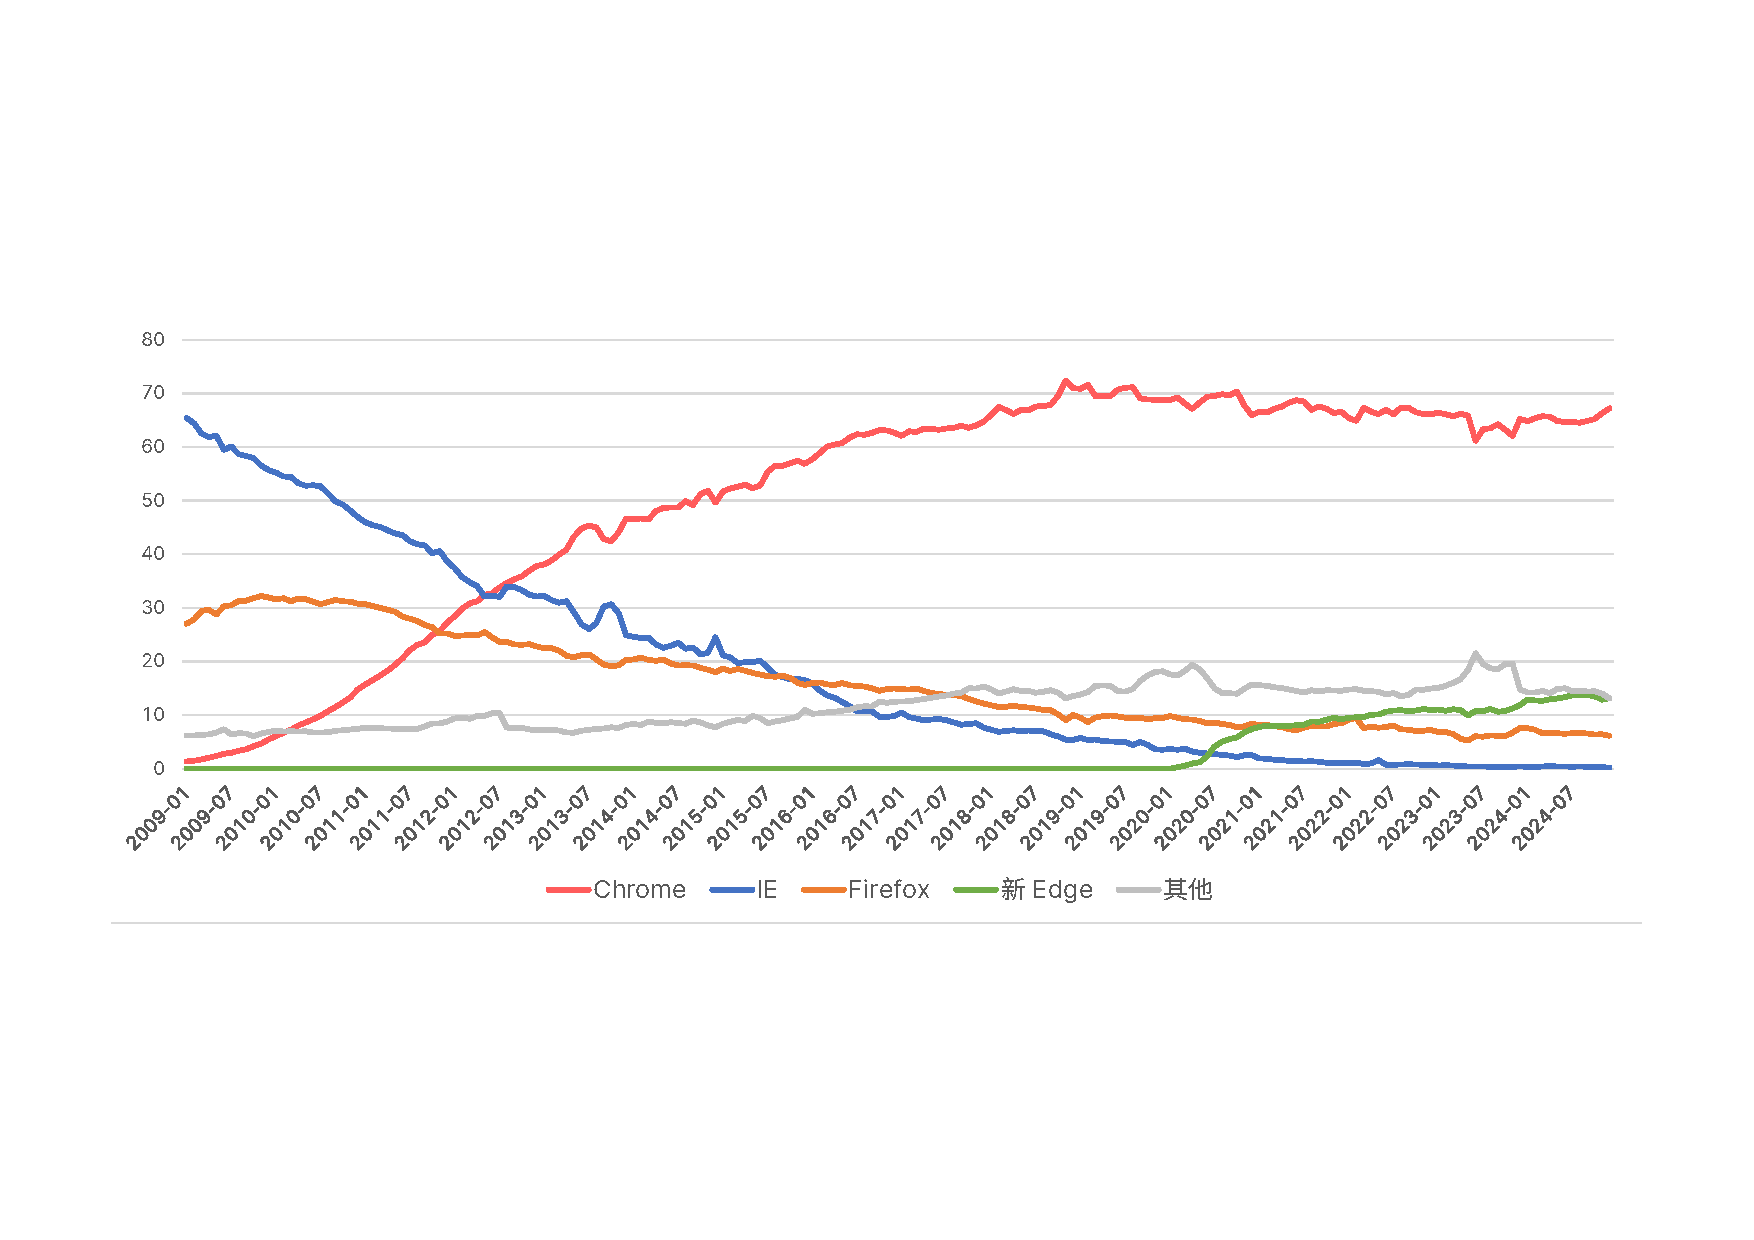
\includegraphics[width=.8\textwidth]{assets/software/Browser_market_share.pdf}
  \caption{电脑端浏览器市场份额}
  \label{fig:Browser_market_share}
\end{figure}

与此同时,Firefox——它使用自己的、不同于 Chromium 的内核——的日子变得不太好过了。在 2010 年之前,Firefox 的市场份额还比较高,且有上升迹象,但在 Chrome 大行其道后就开始逐步下降。虽说 Firefox 在性能上不差,但有时候比不过 Chrome,再加上 Mozilla 毕竟是「用爱发电」,在宣传等方面肯定不如谷歌以及那些套壳大厂来得猛。如今,Firefox 只剩下不到 10\% 的市场占有率。

\regcolor{第二次浏览器大战的余波至今仍未平息,并且是以 Chrome 的碾压性胜利在继续。}在这 20 年间,我们见证了 IE 的衰亡、Edge 的新生、Firefox 的起伏、Chrome 的高歌;以及谷歌的迅速入市、发展和壮大,微软的不断尝试、碰壁和迂回。在互联网时代,市场需求瞬息万变,科技进步日新月异,浏览器之间的竞争背后,实则是技术和资本的较量。未来何去何从我们不得而知,但希望你读到这里时没有昏昏欲睡。

\section{Chrome:一直被模仿,从未被超越}

Chromium 套壳千千万,但我们始终最推荐 Chrome 自身,正所谓「一直被模仿,从未被超越」。

\begin{figure}[htb!]
  \centering
  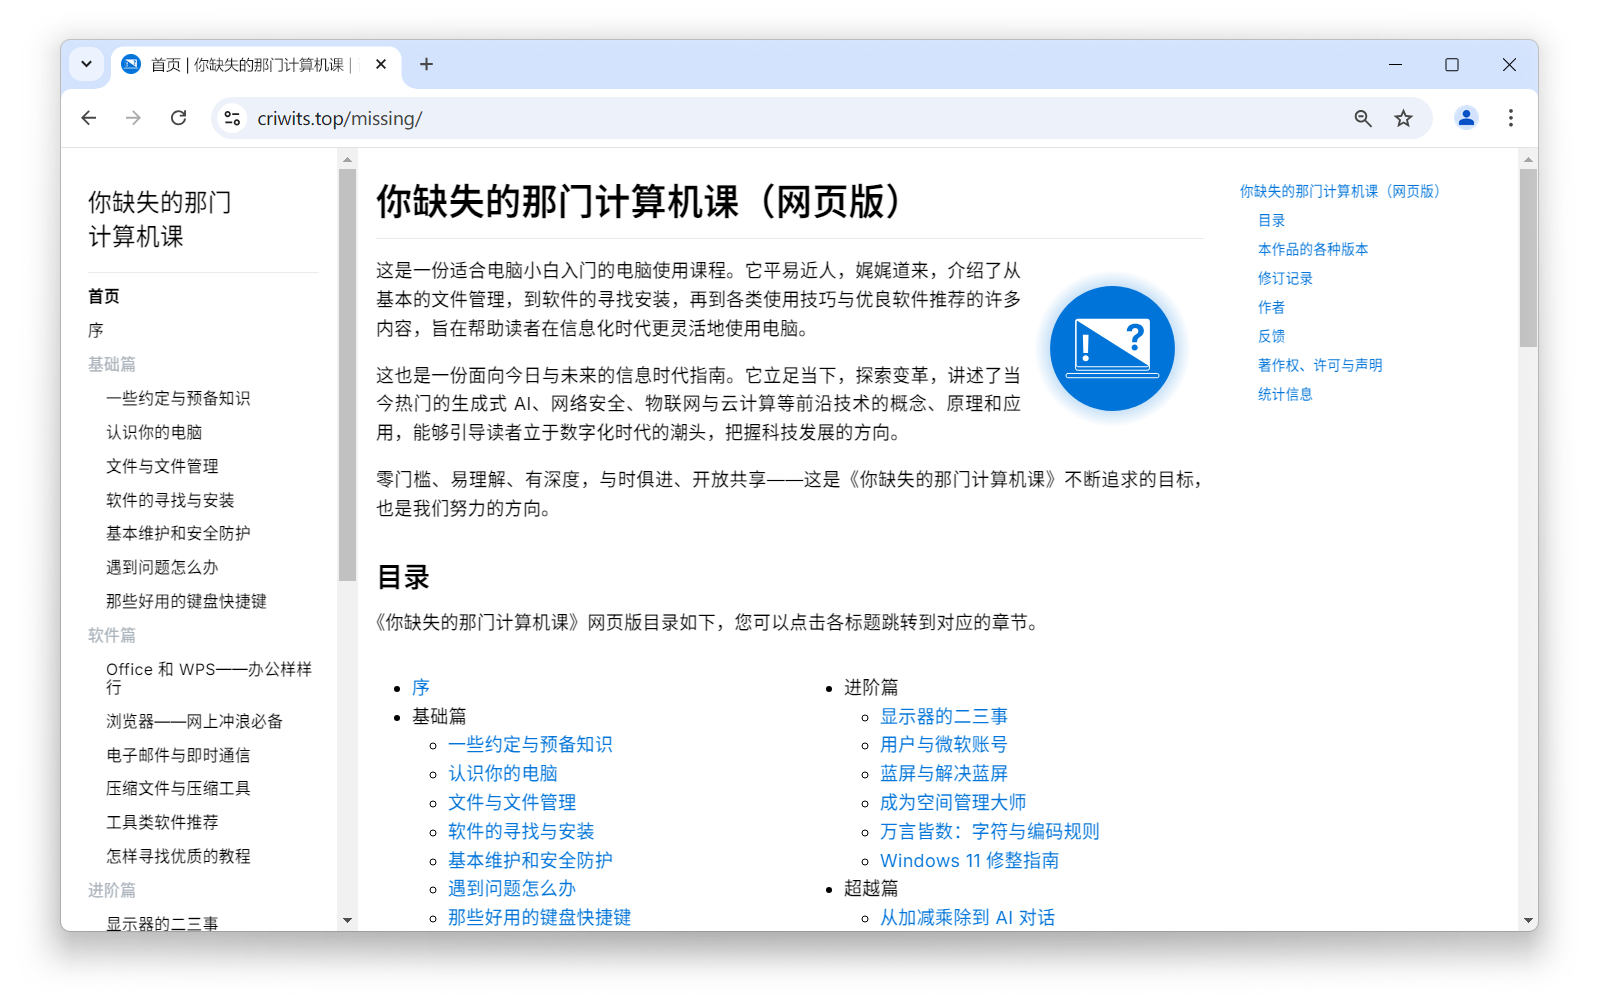
\includegraphics[width=.75\textwidth]{assets/software/Missing_homepage_in_Chrome.png}
  \caption{Chrome}
  \label{fig:Missing_homepage_in_Chrome}
\end{figure}

Chrome 性能出色,界面干净简洁,没有多余繁杂的功能栏,设计优雅美观。Chrome 稍微影响使用的缺点,可能是在内地无法稳定地使用「同步」等功能。这「同步」功能,是指在浏览器上登录自己的账号之后,就能同步自己的收藏夹、历史记录、密码本等数据,实现多设备联动。由于 Chrome 的老东家是谷歌,而谷歌服务无法正常在中国内地访问,这造成一般情况下我们只能不登录使用 Chrome。不过,在自己对同步功能依赖不深的情况下,这一缺点也是可以忽略的。

Chrome 浏览器的官方下载地址是 \url{https://www.google.cn/intl/zh-CN/chrome/}。此链接是可以在中国内地直接访问并正常下载的。下载安装之后的 Chrome 也是可以正常在中国内地更新的。\CJKsout*{(难能可贵难能可贵。)}

\section{Firefox:星星之火,正将燎原}

Firefox——或者说火狐——是今天 Chrome 垄断浏览器市场背景之下还在坚守的浏览器之一。

\begin{figure}[htb!]
  \centering
  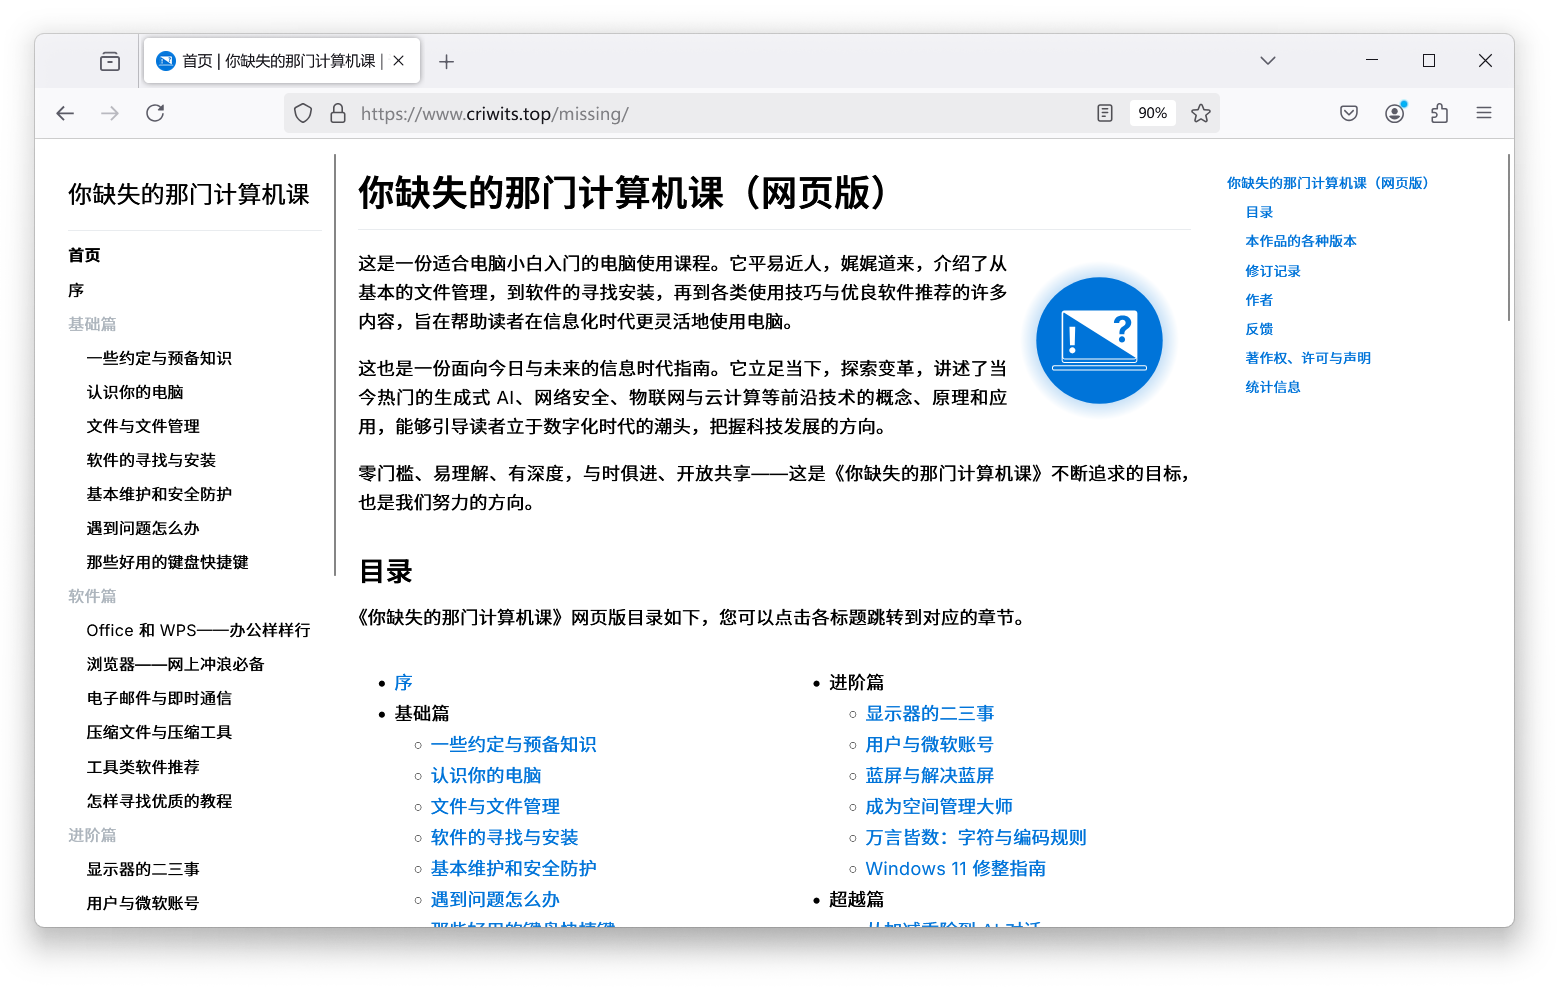
\includegraphics[width=.75\textwidth]{assets/software/Missing_homepage_in_Firefox.png}
  \caption{Firefox}
  \label{fig:Missing_homepage_in_Firefox}
\end{figure}

Firefox 与 Chrome 相当。在界面上,Firefox 同样设计得较为合理美观。\CJKsout*{(怎么它俩长得差不多啊?)}与 Chrome 不同的是,Firefox 可以在国内正常使用同步功能,只需注册一个 Mozilla 账户,即可跨设备同步你的收藏夹、浏览历史等内容。要下载 Firefox,可以直接访问它的官方网站 \url{https://www.firefox.com/}

\begin{note}
  Mozilla 曾与国内的代理公司合作推出过「中国版 Firefox」,它的体验与国际版一致,唯有账号系统与国际版不互通:中国版会将用户的数据存储在中国内地,以遵守数据出境的相关法规。但是,2025 年 7 月底之后,中国版 Firefox 不再提供下载,也不再接受新用户注册,到了 9 月底则完全停止运营,而国际版 Firefox 仍可继续在中国内地使用。
\end{note}

\section{Edge:微软最后的妥协}

这里的「Edge」说的是使用 Chromium 内核的新 Edge,它的图标蓝中带点绿。老 Edge 的图标是蓝色的「e」,不过今天已经不容易见到,因此这里不考虑它。

\begin{figure}[htb!]
  \centering
  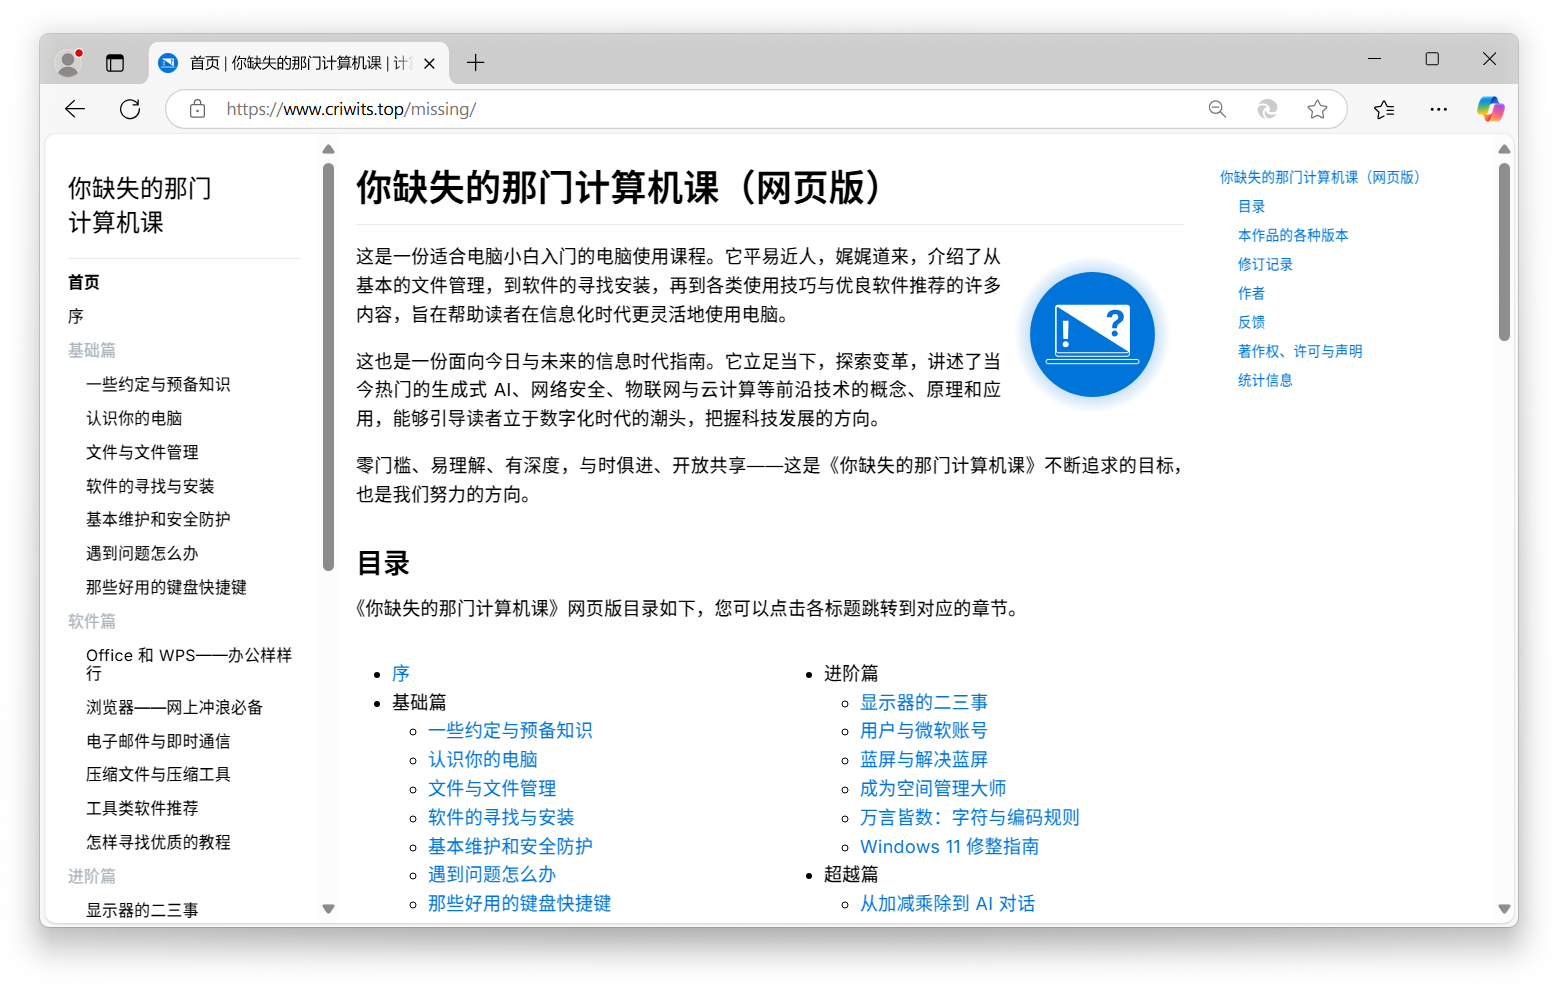
\includegraphics[width=.85\textwidth]{assets/software/Missing_homepage_in_Edge.png}
  \caption{Edge}
  \label{fig:Missing_homepage_in_Edge}
\end{figure}

由于使用了 Chromium 内核,新 Edge 的性能自然和 Chrome 站到了同一梯队。在外观上,新 Edge 和 Chrome 基本一致,但加入了一些比较有用的小功能,例如「垂直标签页」等。\CJKsout*{(怎么它们仨都长得差不多啊?)}Edge 使用微软账号登录,因而也能在国内正常同步。对于想使用 Chrome 却苦于同步等功能的用户来说,新 Edge 是他们非常不错的一个选择。

新 Edge 在现在的 Windows 10 或 11 系统中预置,打开即可使用;如果你想下载安装,可以访问 \url{https://www.microsoft.com/zh-cn/edge}。

\section{IE:也许你还用得到}

\begin{wrapfigure}[9]{r}{6cm}
  \centering
  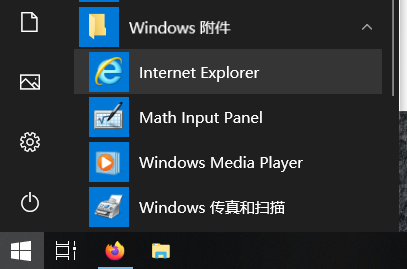
\includegraphics[width=5cm]{assets/software/IE_in_old_Windows_10.png}
  \caption{早期 Windows 10 中的 IE}
  \label{fig:IE_in_old_Windows_10}
\end{wrapfigure}

上文中说过,国内有些网站必须要用 IE 浏览器才能工作。「这样那样的历史原因」便是:这些网站开发得比较早,在那时 IE 还大行其道,因此它们的一些特殊功能(主要是安全相关的功能)是针对 IE 浏览器的部分专有特性开发的。如上文所言,后来斗转星移,IE 最终退出了这个时代,但那些网站却没来得及更新技术。在 2024 年,诸如中国人民银行征信平台、教师资格证报名平台等网站,仍然需要在 IE 浏览器上才能使用完整功能。

在早期的 Windows 10 系统中,IE 11——最后的 IE 版本——得以作为系统的一部分而保留。你可以通过【开始】→【Windows 附件】→【Internet Explorer】来打开它,如\autoref{fig:IE_in_old_Windows_10}。当然你也可以打开「开始菜单」后,直接输入「Internet Explorer」来找到它。

而在 Windows 11,以及最新的 Windows 10 中,IE 已被移出系统。在这种情况下,如果网站要求使用 IE 浏览器,你可以尝试使用 Edge 的「IE 模式」。具体来说,你需要首先打开 Edge 并进入「设置」(右上角【⋯】→【设置】),然后选择【默认浏览器】,将「允许在 Internet Explorer 模式下重新加载网站」设置为【允许】。

\begin{figure}[htb!]
  \centering
  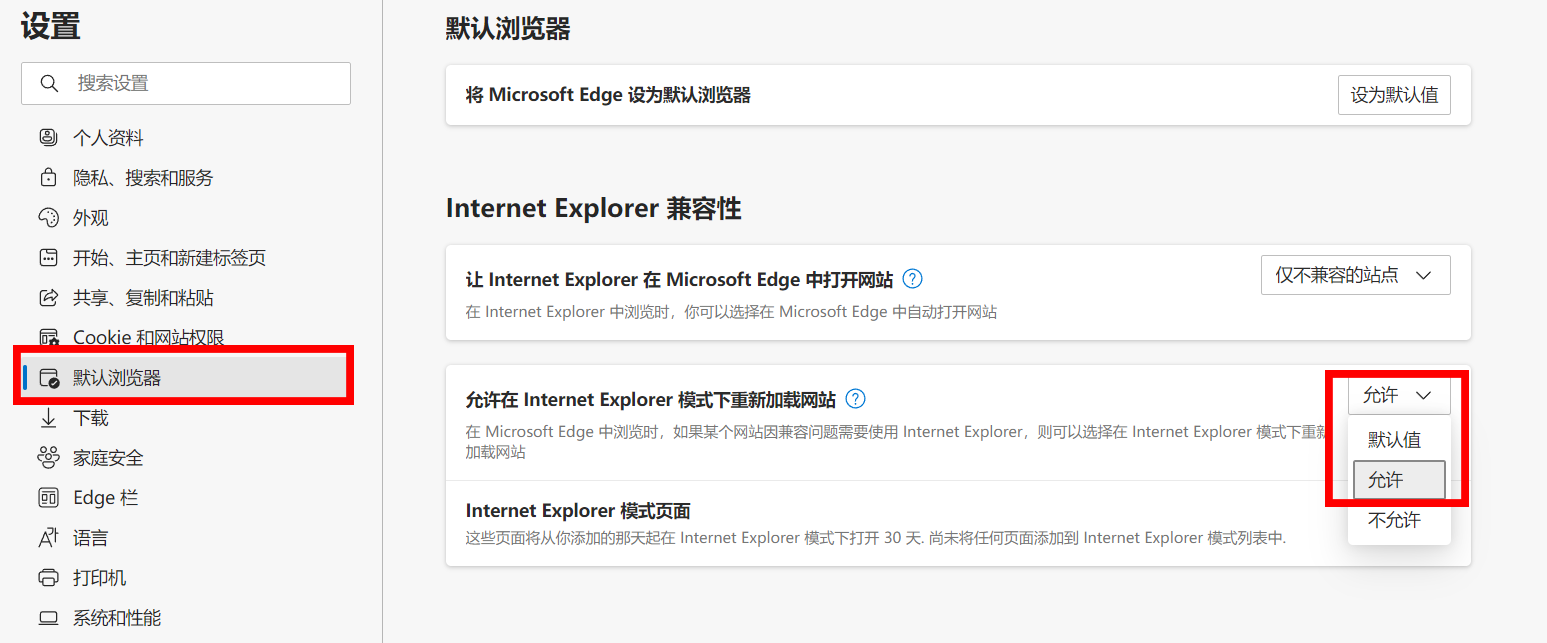
\includegraphics[width=.85\textwidth]{assets/software/Edge_IE_Mode_1.png}
  \caption{启用 Edge 的 IE 兼容}
  \label{fig:Edge_IE_Mode_1}
\end{figure}

设置完之后关闭 Edge 再重新打开。然后,用 Edge 打开你需要用 IE 打开的网页,点击右上角【⋯】并选择【在 Internet Explorer 模式下重新加载】:

\begin{figure}[htb!]
  \centering
  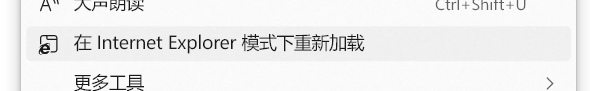
\includegraphics[width=.4\textwidth]{assets/software/Reload_in_IE_mode.png}
  \caption{用 IE 模式重新加载}
  \label{fig:Reload_in_IE_Mode}
\end{figure}

这样网页就相当于是通过 IE 打开了。当然,对于 Windows 10 上的 Edge,也可以用这个方法进入「Internet Explorer 模式」,从而打开那些只支持 IE 浏览器的网站。

\section{国产套壳浏览器:众口难调,各取所需}

最后我们再来说说那些 Chromium 套壳的国产浏览器们。这些浏览器数量庞大,其中不乏优质作品,也有许多劣质软件。一般来说,来自大厂的产品,如「360 安全浏览器」「360 极速浏览器」「QQ 浏览器」和「搜狗高速浏览器」等,通常都具有不错的体验;而那些名不见经传甚至有恶意软件背景的产品,我们十分不建议使用。\autoref{fig:360_se_homepage} 展示的是 360 安全浏览器的官网。如果你习惯使用 360 系列的产品,那么它肯定是适合你的选择。

\begin{figure}[htb!]
  \centering
  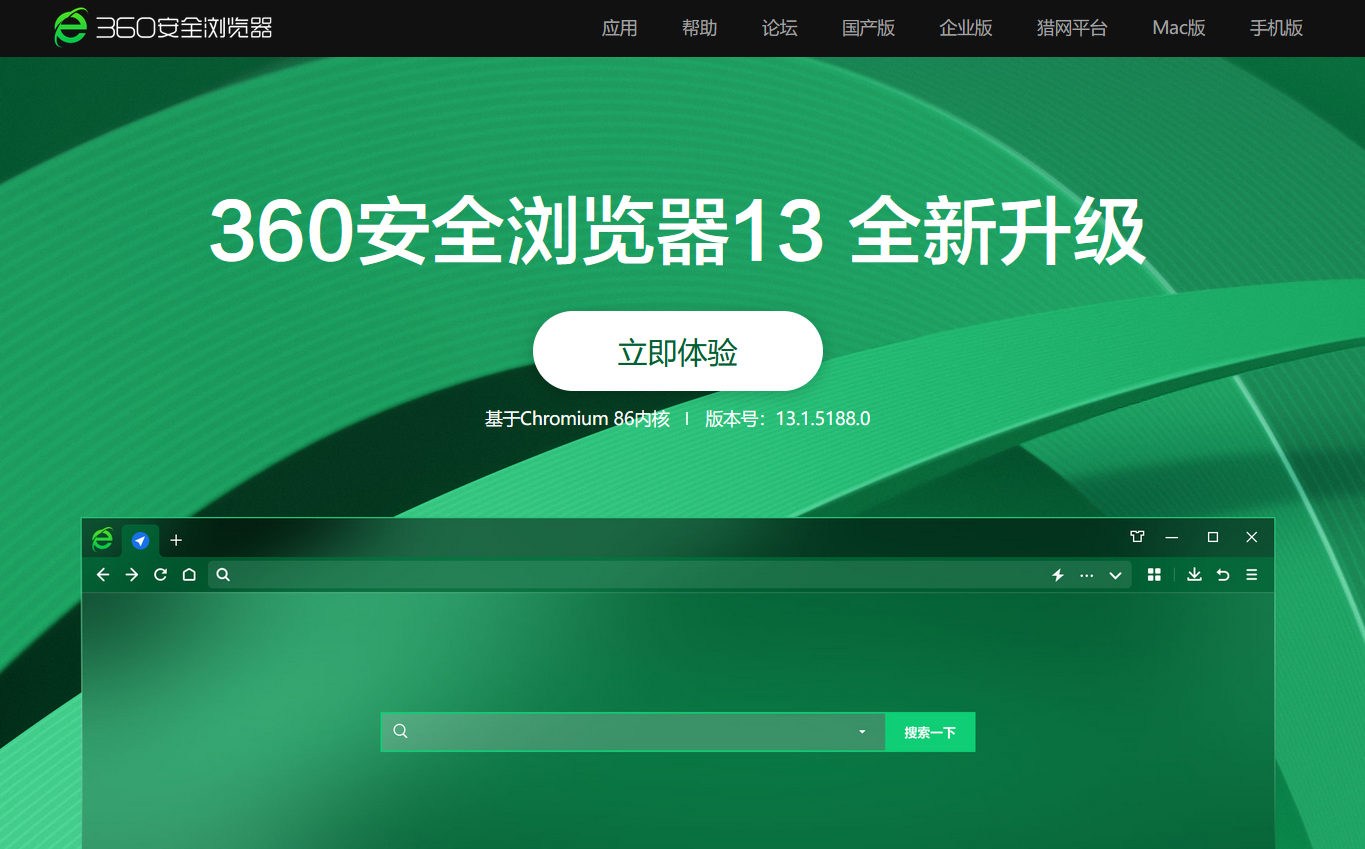
\includegraphics[width=.73\textwidth]{assets/software/360_se_homepage.png}
  \caption{360 安全浏览器的官网}
  \label{fig:360_se_homepage}
\end{figure}

这些国产套壳浏览器有着以下 Chrome 难以提供的功能:

\begin{itemize}
  \item 符合中国用户使用体验的同步功能。这些浏览器使用自家账号(例如 360 账号、QQ/微信号等)登录,往往能与自家产品实现无缝联动,构成完整的体验。
  \item 为国内用户使用习惯打造的资讯推荐功能。这些浏览器一般有自己的首页,而首页上会根据国内用户的使用习惯定制、推荐新闻等推送。民间所谓「UC 体」其实就是 UC 浏览器在首页推送中惯用的一种文体。\CJKsout*{(震惊!这份电脑教程竟如此详细!)}
  \item 各厂商为差异化推出的功能。例如,360 家族的浏览器总是主打「安全」,因为它们的主业是安全产品;QQ 浏览器集成了一些轻度办公的功能,这与腾讯文档等在线办公平台密不可分。
  \item ……
\end{itemize}

但国产套壳浏览器也有着一些令人讨厌之处。首先是国产软件的通病——广告。一些国产套壳浏览器会以弹窗等形式时不时向用户推送广告,这是十分令人厌烦的。另一个问题是它们往往具有「捆绑推荐」的性质,如\chapref{cha:basic-maintenance}中所提到的那样,如果你安装使用 QQ 浏览器,那它总是会在各种场合推荐腾讯的其他软件,比如「腾讯文档」或「腾讯电脑管家」。这很多时候并不是我们所愿意看到的。

总之,对于国产套壳浏览器,我们的建议是「众口难调,各取所需」,大家可以根据自己的实际需要和使用喜好来选用。

\section{设置你的「默认浏览器」}

\begin{wrapfigure}[9]{r}{6.8cm}
  \centering
  \vspace*{-.4cm}
  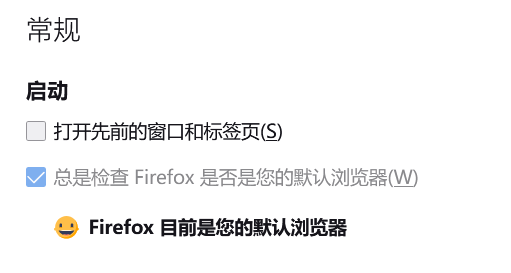
\includegraphics[width=6.3cm]{assets/software/Firefox_default_browser.png}
  \caption{Firefox 的「默认浏览器」设置}
  \label{fig:Firefox_default_browser}
\end{wrapfigure}

所谓「默认浏览器」,是指当你在某处点击一个链接时,系统会自动选择打开它的浏览器。在 \chapref{cha:software-installation}中我们提到了「打开方式」的概念,默认浏览器便是与之类似的东西。

要把一款浏览器设置成你的默认浏览器,大体有两种方式:通过浏览器自身来设置,以及在系统中手动设置。

各大浏览器一般都给出了一键将自己设置成默认浏览器的入口。我们只需要进入浏览器的「设置」「选项」等类似的页面,寻找「默认浏览器」的相关字眼,按提示操作即可完成设置。例如,对于 Firefox,点选【≡】→【设置】就能看到默认浏览器的相关选项。

在系统中手动选择默认浏览器则相对麻烦,不同的系统版本需要不同的操作。在 Windows 11 中,要想在系统中将一款浏览器设置成默认浏览器需要这样操作:

\begin{itemize}
  \item 打开系统【设置】→【应用】→【默认应用】,然后找到你希望设置成默认浏览器的浏览器,如\autoref{fig:Windows_11_default_browser}。
    \begin{figure}[htb!]
      \centering
      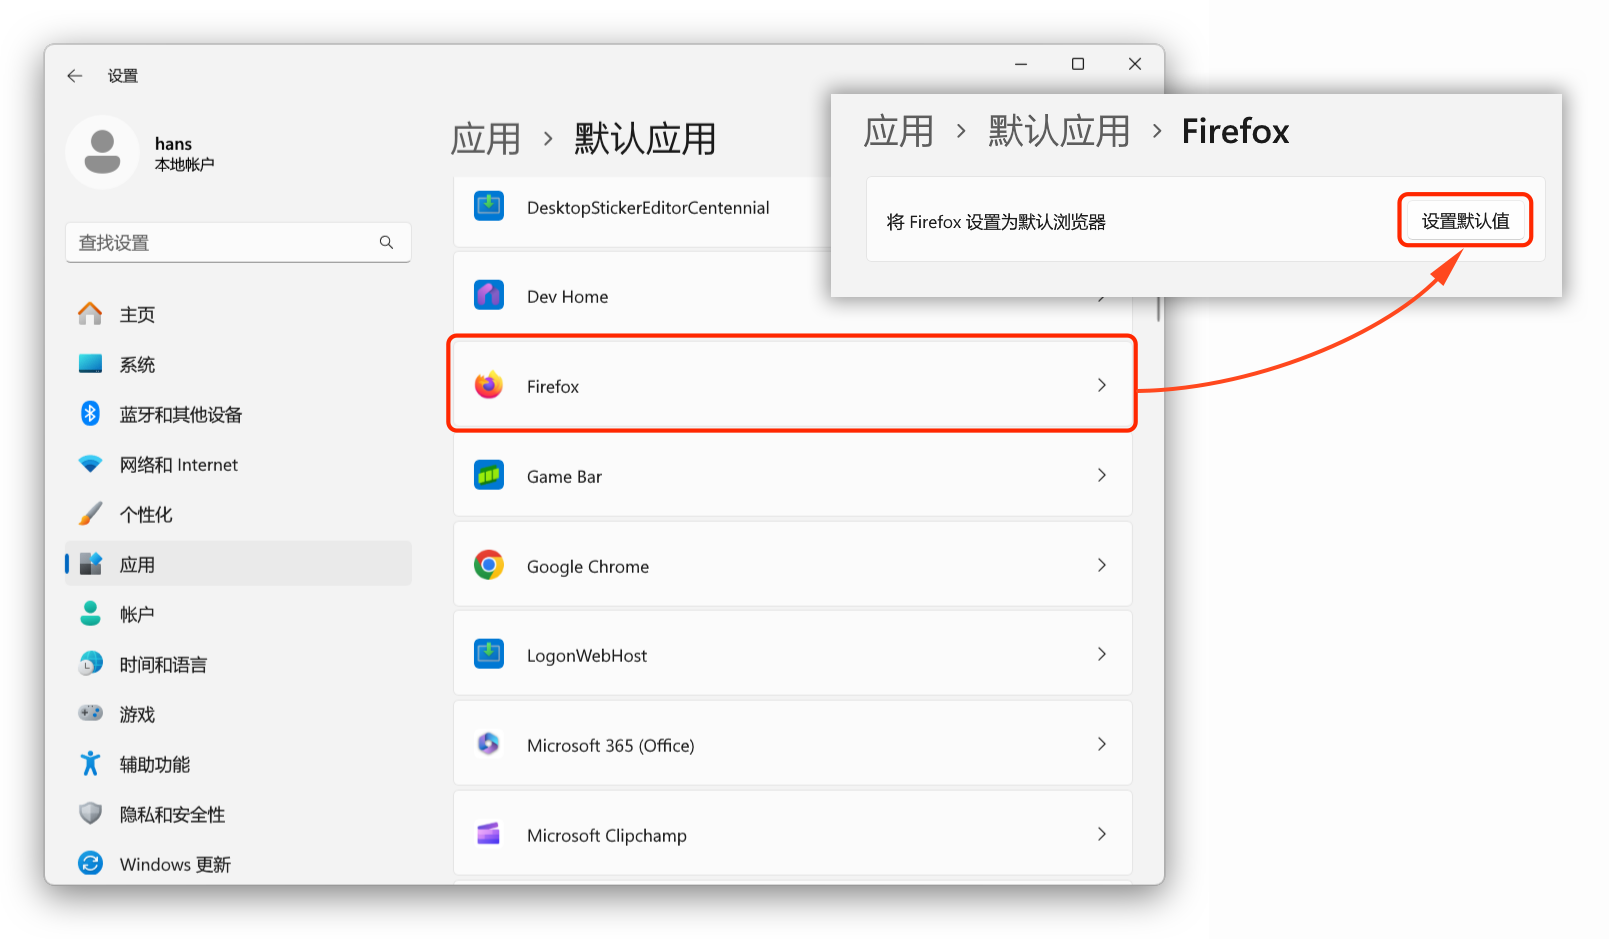
\includegraphics[width=.8\textwidth]{assets/software/Windows_11_default_browser.png}
      \caption{在 Windows 11 中选择默认浏览器}
      \label{fig:Windows_11_default_browser}
    \end{figure}
  \item 点按页面上面的【设置默认值】按钮。如果界面上没有这个按钮,请手动将下面的「\MissingVerb{.htm}」「\MissingVerb{.html}」\linebreak「HTTP」「HTTPS」四个项目修改成你想要的默认浏览器。
\end{itemize}

而在 Windows 10 系统中,你可以通过打开系统【设置】→【应用】→【默认应用】→【Web 浏览器】来选定一款浏览器作为你的默认浏览器,如\autoref{fig:Setting_default_browser}。

\begin{figure}[htb!]
  \centering
  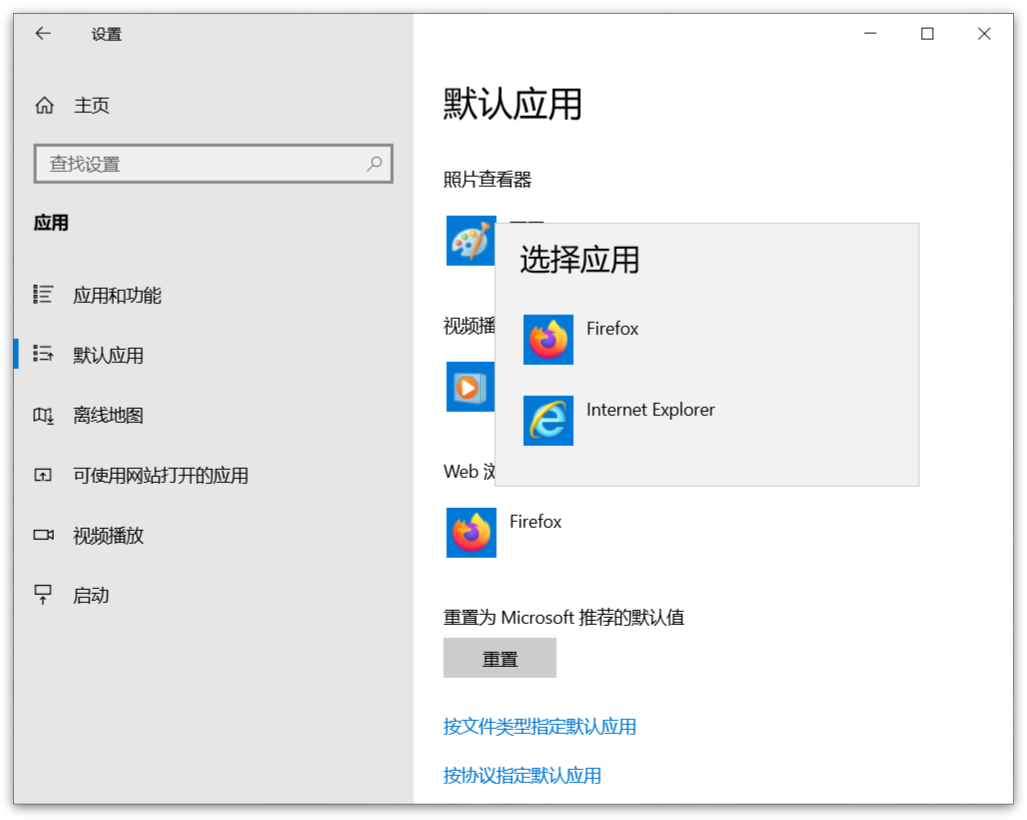
\includegraphics[width=9cm]{assets/software/Setting_default_browser.png}
  \caption{Windows 10 系统的「默认浏览器」设置}
  \label{fig:Setting_default_browser}
\end{figure}

\practice

\begin{enumerate}
  \item 根据「浏览器界的『血雨腥风』」一节的叙述,复述任意一款主流浏览器(Firefox、IE、Chrome)的发展兴衰史。
  \item 你正在用什么浏览器?你喜欢它的什么功能?如果你在阅读完这部分内容后想更换一款浏览器并长久使用,你会选择哪一款?
  \item 电脑里安装的浏览器是越多越好吗?为什么?
\end{enumerate}